\section{Dipole}

Als erstes Thema werden Dipolantennen beschrieben. Dabei wird vor allem auf den Hertzschen Dipol eingegangen, welcher das Modell der Antenne durch seine kurze Länge vereinfacht.

\subsection{Hertzscher Dipol}\label{sec:HerDip}

Eine Dipol Antenne kann als kurzer Linearstrahler beschrieben werden, wobei dessen länge $l \ll \lambda_0 /4$ beträgt. $\lambda_0$ beschreibt dabei die Wellenlänge, welche durch das Verhältnis der Lichtgeschwindigkeit zur Signalfrequenz $c_0/f$ beschreibt. 

xxx

Ein solcher Strahler ist in Abbildung xxx zu sehen, wobei $\underline{I}$ der komplexe Strom einer Sinusschwingung darstellt, welche konstant über die gesamte Länge schwingt. $\phi$ stellt den Winkel dar, welcher um die z-Achse rotiert und über die x- und y-Achse aufgespannt ist.$\theta$ hingegen rotiert um die x-Achse und wird über die y- und z-Achse aufgespannt. Für die Kugelkoordinaten bedeutet dies, dass mit den Restriktionen 

\begin{align}
&0 \leq \varphi \leq 2\pi\\
&0 \leq \vartheta \leq \pi \label{eq:HertzTheta}
\end{align}

der gesamte Bereich des Koordinatensystems abgedeckt ist. Das durch den Strom induzierte Magnetfeld kann mit 

\begin{equation}
\underline{H}_0 = j\pi \frac{\underline{I}l}{{\lambda_0}^2}
\end{equation}

beschrieben werden, was für zwei Formeln für das magnetische und elektrische Feld liefert:

\begin{align}
\underline{H}_\varphi   &= \underline{H}_0 \sin \vartheta \frac{e^{-jk_0r}}{k_0r}\\
\underline{E}_\vartheta &= Z_0 \underline{H}_\varphi = Z_0 \underline{H}_0 \sin \vartheta \frac{e^{-jk_0r}}{k_0r}.\label{eq:HertzE}
\end{align}

Hierbei beschreibt $r$ die Distanz des Punktes zu Ursprung und $k_0 = \omega \sqrt{\mu_0 \eta_0} = c_0/\omega$ die Wellenzahl im Vakuum beschreibt. Somit beschreibt die komplexe Exponentialfunktion die Ausbreitung der Welle, was mit der Theorie der Wellenleitern übereinstimmt. Im Nenner ist das Abklingen des Sinus zu erkennen, welches abhängig von der Distanz zum Ursprung und der Wellenzahl ist. xxx

\subsection{Richtdiagramm}

Ein wichtiges Diagramm für die Analyse von Antennen ist das Richtdiagramm. Mit diesem kann die Direktivität einer Antenne dargestellt werden, welche mitteilt, in welche Richtung wie viel der Leistung der Antenne abgestrahlt wird. Diese Analyse geschieht im Fernfeld, was bedeutet dass die Annahme $r \rightarrow \infty$ getroffen wird. Somit kann verhindert werden, dass eine Antenne in eine unerwünschte Richtung Leistung abgibt und somit eine andere Antenne stören könnte. Daher wird die Feldstärke einer Antenne in Abhängigkeit der Raumrichtung beschreiben, welche mit den Kugelkoordinaten $\varphi$ und $\vartheta$ angegeben wird.\\

Für das Richtdiagramm wird die komplexe elektrische Feldstärke in den Kugelkoordinaten auf dessen maximale Feldstärke normiert, wobei sich dadurch ein wert zwischen $0$ und $1$ einstellt. Dies ergibt die auf den Maximalwert normierte Winkelverteilung des elektrischen Feldes. Diese Kenngrösse wird als Richtcharakteristik bezeichnet:

\begin{equation}
C(\vartheta,\varphi) = \frac{|\underline{E}(\vartheta,\varphi)|}{|\underline{E}(\vartheta,\varphi)|_{\mathrm{max}}}.
\end{equation}

Als Beispiel wird der Hertzsche Dipol aus dem Abschnitt \ref{sec:HerDip} betrachtet. Dessen elektrische Feldstärke ist in Formel \ref{eq:HertzE} beschrieben, wobei durch den Sinus dessen Maximalwert direkt bestimmt werden kann. Somit ergibt sich für die Richtcharakteristik:

\begin{equation}\label{eq:HertRicht}
C(\vartheta,\varphi) = \frac{|\underline{E}(\vartheta,\varphi)|}{|\underline{E}(\vartheta,\varphi)|_{\mathrm{max}}} = \frac{\frac{Z_0 |\underline{H}_0| |\sin \vartheta|}{k_0r}}{\frac{Z_0 |\underline{H}_0|}{k_0r}} = \sin \vartheta.
\end{equation}

Aus Formel \ref{eq:HertRicht} ist herauszulesen, dass an der Stellen für $\vartheta$ gleich Null oder $\pi$ eine Nullstelle ist, das Maximum an der Stelle $\pi/2$ mit dem normierten Wert 1 erreicht wird und bei $\pi/4$ der Wert $1/\sqrt{2}$ anliegt.\\

Zur Verifikation wurde zuerst ein MATLAB-Code erstellt, welcher die Polarkoordinaten darstellen soll.

\begin{lstlisting}
%Richtcharakteristik.m

%Thomas Frei & Simon Zoller

%Kugelkoordinaten
theta=0:0.01:2*pi;
phi = 0:0.01:2*pi;

%Richtcharakteristik
C = cell(6);

%Titel
plotTitle = cell(6);
plotTitle{1} = 'Vertikales Richtdiagramm z-Dipol';
plotTitle{2} = 'Horizontales Richtdiagramm z-Dipol';
plotTitle{3} = 'Vertikales Richtdiagramm x-Dipol';
plotTitle{4} = 'Horizontales Richtdiagramm x-Dipol';
plotTitle{5} = 'Vertikales Richtdiagramm y-Dipol';
plotTitle{6} = 'Horizontales Richtdiagramm y-Dipol';

%z-Dipol
C{1} = abs(sin(theta));
C{2} = ones(size(theta));

%x-Dipol
C{3} = abs(sqrt(1-sin(theta).^2.*cos(pi/2).^2));
C{4} = abs(sqrt(1-sin(pi/2).^2.*cos(phi).^2));

%y-Dipol
C{5} = abs(sqrt(1-sin(theta).^2.*sin(pi).^2));
C{6} = abs(sqrt(1-sin(pi/2).^2.*sin(phi).^2));

%Plot in Schleife
for ind=1:6
    subplot(3, 2, ind) ;
    polarplot(theta,C{ind});
    pax = gca;
    pax.ThetaDir = 'clockwise';
    pax.ThetaZeroLocation = 'top';
    rlim([0 1]);
    title(plotTitle{ind});
end
\end{lstlisting}

\begin{figure}[!ht]
	\centering
    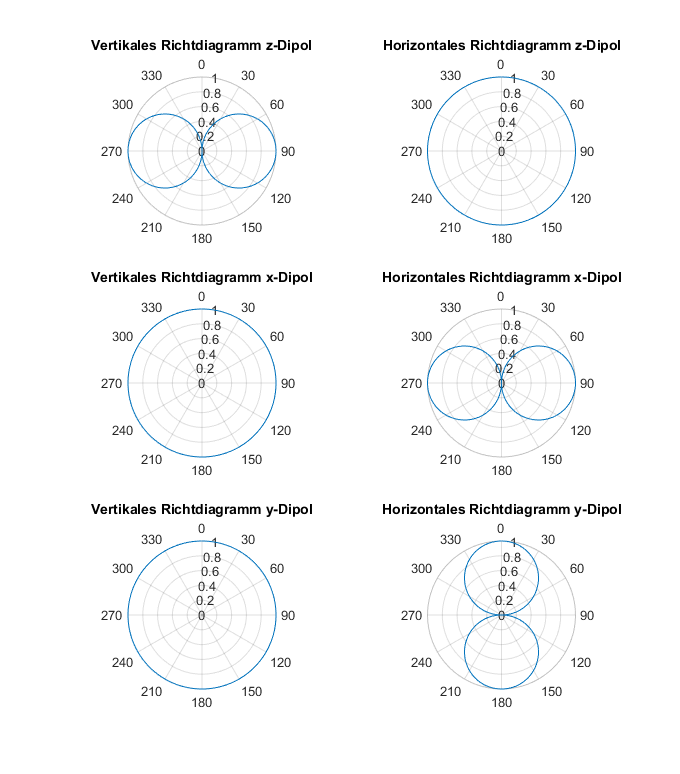
\includegraphics[width=\textwidth]{HertzscherDipol.png}
    \caption{Simulationen des Hertzschen Dipoles mit der Anordnung in allen drei verschiedenen Achsenrichtungen.}
    \label{fig:HertzscherDipol}
\end{figure}

Das Resultat ist in Figur \ref{fig:HertzscherDipol} zu sehen. Die Werte stimmen mit den Annahmen überein und auch mit der erwarteten Figur xxx. Zu beachten ist jedoch, dass nur ein Kreis ersichtlich ist, da wie in Formel \ref{eq:HertzTheta} definiert $\vartheta$ nur über den halben Bereich gilt. Das Resultat in Figur xxx ist dreidimensional angegeben. Meistens reicht es jedoch, einen Schnitt der Charakteristik anzugeben. Dabei wird unter dem vertikalen und horizontalen Richtdiagramm unterschieden, wobei für das vertikale Diagramm mit $C(\vartheta, \varphi = \varphi_0)$ die Strahlung im Elevationswinkel $\vartheta$ angegeben wird (wie in Figur xxx) und beim horizontalen Diagramm mit $C(\vartheta=\pi/2, \varphi)$ die Strahlung im sogenannten Azimutwinkel $\varphi$ angegeben wird. Dies resultiert in der E-Ebene für das vertikale Diagramm und in der H-Ebene für das horizontale Diagramm des z-Dipols.\\

Als letzter Teil der Theorie wird auf die Halbwertsbreiten $\Delta \vartheta$ und $\Delta \varphi$ eingegangen. Diese beschreiben die Breite der Hauptkeule, wobei der Winkel unter welchem die Hälfte der Strahlungsdichte liegt angegeben wird (beziehungsweise der -3dB Punkt). Da wie schon erwähnt beim Hertschen Dipol bei $\pi/4$ die Richtcharakteristik $1/\sqrt{2}$ beträgt, ergibt sich für die Halbwertsbreiten einen Winkel von \SI{90}{\degree}.

\subsection{Linearantenne}

Eine Linearantenne ist ein Typ Antenne, welche eine Länge um die Grösse $\lambda_0/2$ besitzt. Diese werden umgänglich für Mittel- und Langwellen Anwendungen gebraucht wegen ihrer Einfachheit. Die Antenne besteht aus einem geraden, zylindrischen Leiter, welcher einen dünnen Durchmesser besitzt. Dabei gilt, dass der Schlankheitsgrad

\begin{equation}
s = \frac{l}{d}=\frac{2h}{d} \geq 75
\end{equation} 

beträgt und der Durchmesser

\begin{equation}
d \leq \frac{\lambda_0}{50}
\end{equation}

erfüllt. Somit kann für die Berechnung der Felder die Integration über eine Hüllfläche durch eine eindimensionale Integration vereinfacht werden, was den Rechenaufwand erleichtert.\\
Die lineare Antenne kann auf zwei Arten gespiesen werden. Entweder wird die Antenne als Monopol betrieben und am Fusspunkt gegen Erde erregt, oder sie wird in der Mitte als Monopol symmetrisch erregt. Bei der Dipol Ausführung ist jedoch ein Spalt in der Mitte notwendig, welcher vernachlässigbar klein sein soll. Die beiden Anordnungen unterscheiden sich nicht im Strahlungsdiagramm da die Erdoberfläche die Symmetrieebene des elektrischen Feldes darstellt. Der Monopol, welcher halb so lang wie der Dipol gewählt wird, gibt bei einem identischen Speisestrom gerade die halbe Strahlungsleistung ab, was zu einem doppelten Gewinn führt.\\

Für die Simulationen interessierten uns die Richtdiagramme der Linearantennen. Dazu wurde der Halbwellendipol, der Ganzwellendipol und der Doppelwellendipol betrachtet. Dabei wurde die Herleitung der Richtcharakteristik weggelassen, da uns hauptsächlich die Simulationsresultate interessieren.\\

Der Halbwellendipol besitzt eine Antennenlänge von $\lambda_0/2$, was zu einer Richtcharakteristik von 

\begin{equation}\label{eq:RichtHalb}
C(\vartheta) = \frac{\cos \left(\frac{\pi}{2}\cos \vartheta \right)}{\sin \vartheta}.
\end{equation}

Die Richtcharakteristik des Ganzwellendipols beträgt bei dessen Antennenlänge von $\lambda_0$

\begin{equation}
C(\vartheta) = \frac{\cos^2 \left(\frac{\pi}{2}\cos \vartheta \right)}{\sin \vartheta}.
\end{equation}

Der Doppelwellendipol ist $2\lambda_0$ lang und dessen Richtcharakteristik beträgt:

\begin{equation}\label{eq:RichtDoppel}
C(\vartheta) = \frac{\sin^2 \left(\pi \cos \vartheta \right)}{\sin \vartheta}.
\end{equation}

\begin{figure}[!ht]
	\centering
    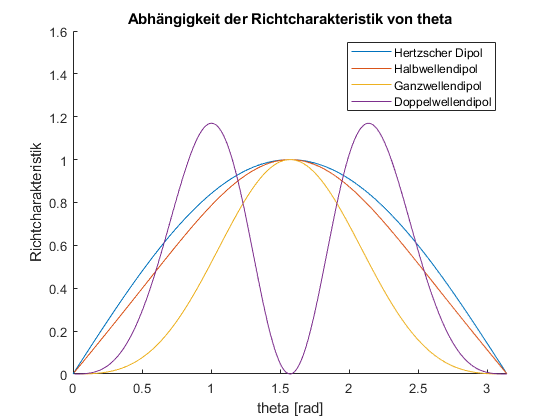
\includegraphics[width=\textwidth/4*3]{Wellendipol.png}
    \caption{Ein Plot der jeweiligen Richtcharakteristiken verschiedener Linearantennen.}
    \label{fig:Wellendipol}
\end{figure}

In Abbildung \ref{fig:Wellendipol} ist die Richtcharakteristik der Antennen in Abhängigkeit von $\vartheta$ zu sehen. Dabei wurde der Hertzsche Dipol auch eingefügt, um die Richtdiagramme besser vergleichen zu können. Wie sich erkennen lässt, besitzt der Hertzsche Dipol die grösste Halbwertsbreite von allen Antennen. Beim Halbwellendipol ist diese nur leicht kleiner, wobei sich beim Ganzwellendipol eine bemerkbar kleinere Halbwertsbreite einstellt. Dabei liegen die -3dB Punkte bei \num{1.99} und \num{1.15} welche einen Winkel von \SI{48}{\degree} ergeben. Dieser beträgt fast halb so viel wie die \SI{90}{\degree} Halbwertsbreite des Hertzschen Dipols. Der Doppelwellendipol besitzt sogar eine Nullstelle bei $\pi/2$, wo sich die Maximalwerte der anderen Antennen befinden. Der Maximalwert des Doppelwellendipols liegt jedoch bei \num{1} und \num{2.14}, was einen Maximalwert bei \SI{57.3}{\degree} und \SI{122.6}{\degree} ergibt. Dabei wird klar, dass das dazugehörige Richtdiagramm vier Keulen besitzen wird.\\

\subsection{Simulation}

Im Buch von xxx auf Seite 249 befindet sich eine Tabelle mit den Richtdiagrammen der obigen genannten linearen Antennen. Dabei wurde die Länge der jeweiligen Antenne noch mit dem Faktor n angepasst, was uns aus den Formeln \ref{eq:RichtHalb} bis \ref{eq:RichtDoppel} folgende Längen und Richtcharakteristiken ergeben:

Für den Halbwellendipol:

\begin{align}
l &= (2n-1)\frac{\lambda_0}{2}\\
C(\vartheta) &= \frac{\cos \left(\frac{2n-1}{2}\pi \cos \vartheta \right)}{\sin \vartheta}
\end{align} 

Für den Ganzwellendipol:

\begin{align}
l &= (2n-1)\lambda_0\\
C(\vartheta) &= \frac{\cos^2 \left(\frac{2n-1}{2}\pi \cos \vartheta \right)}{\sin \vartheta}
\end{align} 

Für den Doppelwellendipol:

\begin{align}
l &= (2n\lambda_0\\
C(\vartheta) &= \frac{\sin^2 \left(n \pi \cos \vartheta \right)}{\sin \vartheta}
\end{align} 

Für die Simulation wurde ein Dipol aufgebaut mit entsprechender Länge, welche für die Anregung ein Vakuum mit vernachlässigbarer Länge besitzen, in welchem sich der Anregungsport befindet. Für die Simulation wurde das Standard Anregungssignal verwendet und als Frequenz wurde \SI{1}{\giga\hertz} verwendet. Die Datei wurde so geschrieben, dass alle Antennentypen mit minimalem Aufwand simuliert werden können, ohne dass das Modell abgeändert werden muss. 

\begin{figure}[!ht]
	\centering
    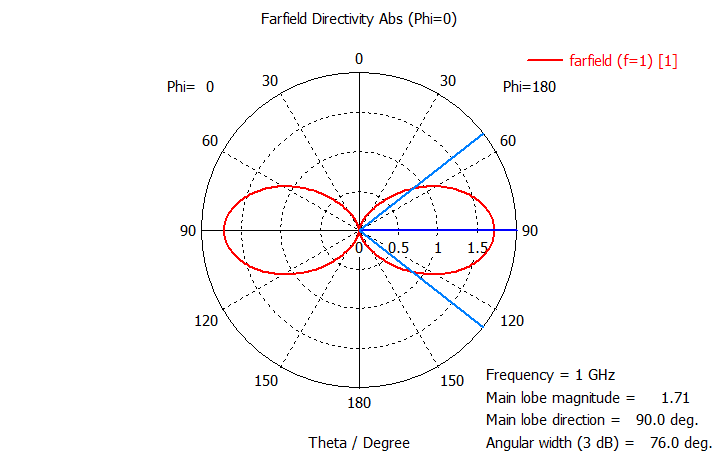
\includegraphics[width=\textwidth]{Halbwellendipol1.png}
    \caption{Direktivität der Halbwellendipolantenne.}
    \label{fig:Halbwellendipol1}
\end{figure}

In Abbildung \ref{fig:Halbwellendipol1} ist das Richtdiagramm des Halbwellendipols zu sehen. Wie bereits erwähnt ist dessen Halbwertsbreite leicht kleiner als \SI{90}{\degree} welche bei $\vartheta = 90^\circ$ am stärksten abgestrahlt wird.

\begin{figure}[!ht]
	\centering
    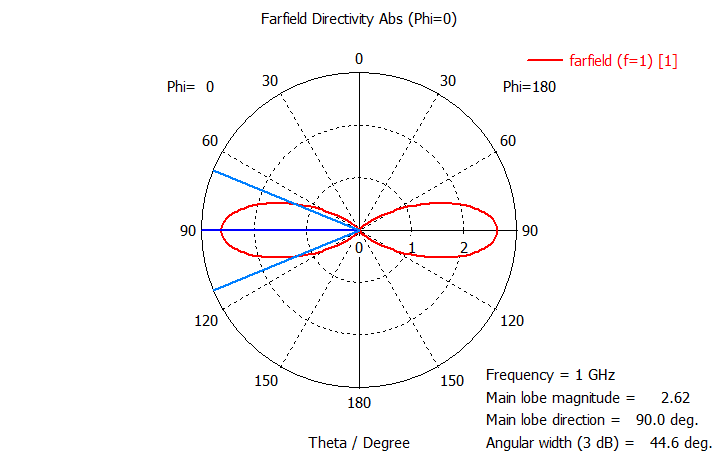
\includegraphics[width=\textwidth]{Ganzwellendipol1.png}
    \caption{Richtdiagramm des Ganzwellendipoles.}
    \label{fig:Ganzwellendipol1}
\end{figure}

Abbildung \ref{fig:Ganzwellendipol1} zeigt die Direktivität des Ganzwellendipols. Berechnet wurde dabei eine Halbwertsbreite von \SI{48}{\degree} und simuliert wurde eine Halbwertsbreite von \SI{44.6}{\degree}. Diese Abweichung ist minimal, weshalb die Simulation als erfolgreich verifiziert werden kann. Auch hier ist die maximale Leistungsabgabe identisch mit dem vorherigen Resultat.

\begin{figure}[!ht]
	\centering
    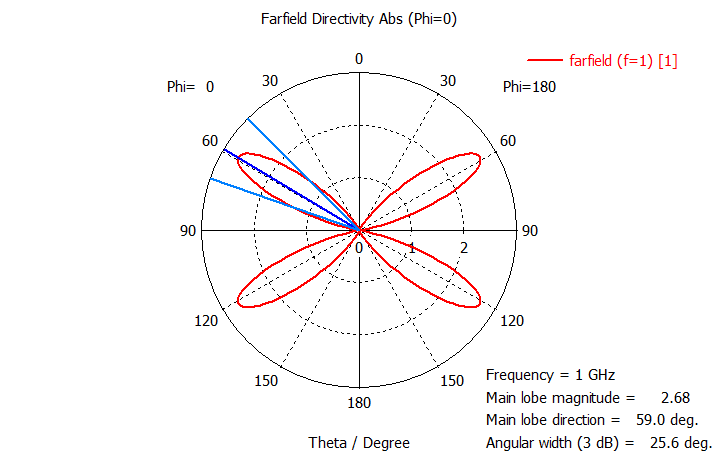
\includegraphics[width=\textwidth]{Doppelwellendipol1.png}
    \caption{Resultat der Simulation des Doppelwellendipols.}
    \label{fig:Doppelwellendipol1}
\end{figure}

Wie in Abbuldung \ref{fig:Doppelwellendipol1} zu sehen ist, verhält sich das Richtdiagramm wie berechnet wurde. Es entstehen vier Keulen, wobei der Winkel bei der Simulation \SI{59}{\degree} beträgt anstelle der berechneten \SI{57.3}{\degree}. Dies ist auch wiederum eine vernachlässigbar kleine Abweichung.

\begin{figure}[!ht]
	\centering
    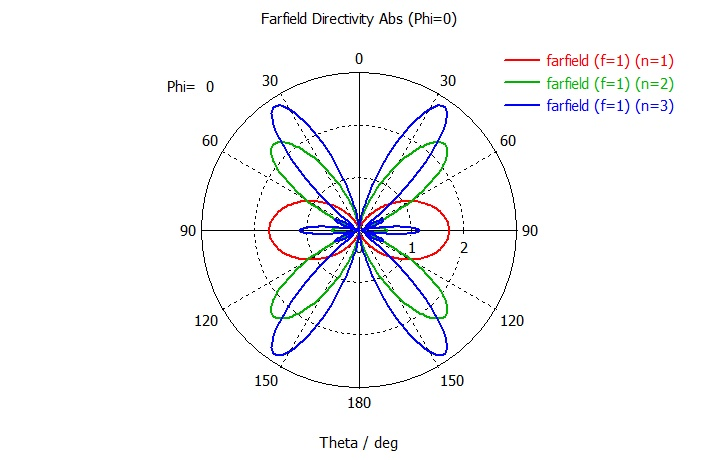
\includegraphics[width=\textwidth]{Halbwellendipol13.jpg}
    \caption{Direktivität der Halbwellendipolantenne mit $n = 1 ... 3$.}
    \label{fig:Halbwellendipol13}
\end{figure}

\begin{figure}[!ht]
	\centering
    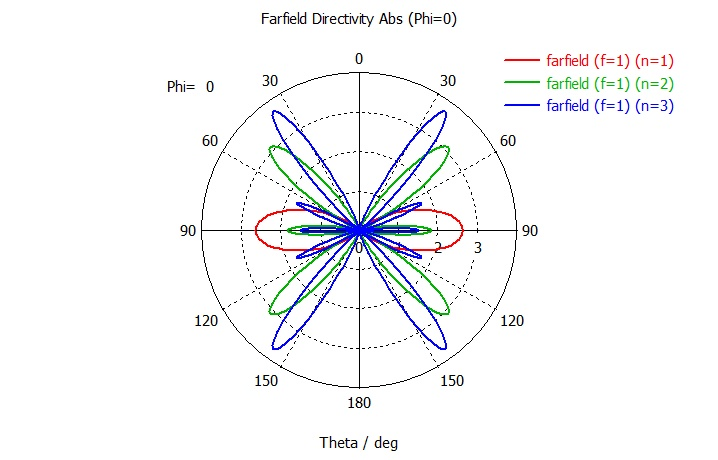
\includegraphics[width=\textwidth]{Ganzwellendipol13.jpg}
    \caption{Richtdiagramm des Ganzwellendipoles mit $n = 1 ... 3$.}
    \label{fig:Ganzwellendipol13}
\end{figure}

\begin{figure}[!ht]
	\centering
    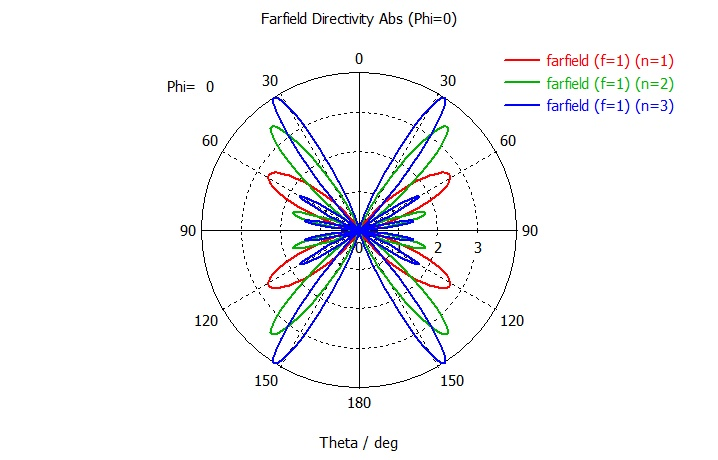
\includegraphics[width=\textwidth]{Doppelwellendipol13.jpg}
    \caption{Resultat der Simulation des Doppelwellendipols mit $n = 1 ... 3$.}
    \label{fig:Doppelwellendipol13}
\end{figure}

Als Abschluss der linearen Antenne wurden in Abbildungen \ref{fig:Halbwellendipol13} bis \ref{fig:Doppelwellendipol13} die höheren Ordnungen für $n$ simuliert. 

xxx

\begin{figure}[!ht]
	\centering
    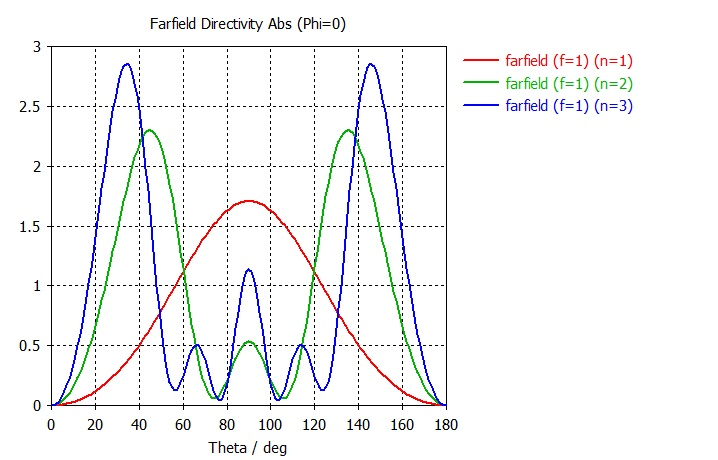
\includegraphics[width=\textwidth]{Halbwellendipol13Cart.jpg}
    \caption{Direktivität der Halbwellendipolantenne mit $n = 1 ... 3$ in kartesischen Koordinaten.}
    \label{fig:Halbwellendipol13Cart}
\end{figure}

Natürlich kann auch im Vergleich zu Abbildung \ref{fig:Wellendipol} das Resultat in Kartesichen Koordinaten dargestellt werden. Dies resultiert in Abbildung \ref{fig:Halbwellendipol13Cart}. Somit stellt diese Abbildung dasselbe Resultat wie Abbildung \ref{fig:Halbwellendipol13} dar, wobei bei den kartesischen Koordinaten das Herauslesen der Halbwertsbreite etwas einfacher ist. Bei den Kugelkoordinaten fällt es hingegen leichter, sich die Abstrahlunsrichtungen vorzustellen.

\begin{figure}[!ht]
	\centering
    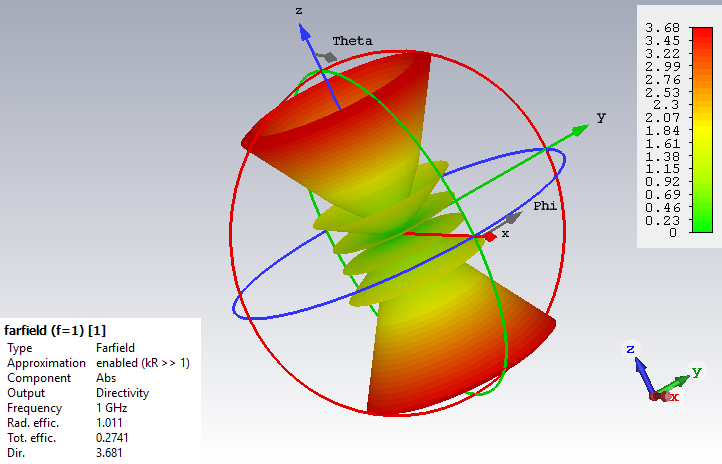
\includegraphics[width=\textwidth]{3D.png}
    \caption{Darstellung des Doppelwellendipols mit $n = 3$ in dreidimensionalen Koordinaten.}
    \label{fig:3D}
\end{figure}

Dabei zeigt Abbildung \ref{fig:3D} die dreidimensionale Direktivität. Es ist ausserdem zu sehen, wie die Antenne geschnitten wurde, um das Richtdiagramm darzustellen. Es ist wichtig zu wissen, dass verschiedene Antennen in andere Richtungen abstrahlen und daher der Schnittwinkel angepasst werden muss (vergleichsweise Hetzscher Dipol entlang der verschiedenen Achsen in Abschnitt xxx).

\subsection{Simulationen}

